\documentclass[12pt,a4paper]{article}

\usepackage[utf8]{inputenc}
\usepackage[T1]{fontenc}
\usepackage[brazilian]{babel}
\usepackage{amsmath}
\usepackage{graphicx}
\usepackage{geometry}
\usepackage{float}
\usepackage{hyperref}

\geometry{top=2.5cm, bottom=2.5cm, left=3cm, right=3cm}

\title{Atividade 2: Adaline \\ \large Disciplina: Redes Neurais Artificiais}
\author{Programa de Pós-Graduação em Ciência da Computação (PPGCC-UNESP)}
\date{\today}

\begin{document}

\maketitle

\section{Introdução e Implementação}
Este documento apresenta os resultados da implementação e avaliação do modelo ADALINE (Adaptive Linear Neuron). A implementação foi baseada no algoritmo do Perceptron, adaptando a regra de atualização dos pesos para utilizar o erro contínuo e minimizar o Erro Quadrático Médio ($E_{qm}$).

O algoritmo foi implementado suportando duas abordagens de treinamento, por amostra e por batch.

O bias foi fixado em 1 e inserido tanto nos vetores de entrada quanto inicializado de forma aleatória no vetor de pesos.

\section{Experimentos: Dataset 1}
O primeiro experimento foi conduzido em uma base de 2 atributos, com 140 amostras de treino e 60 amostras de teste. Os parâmetros utilizados foram: limite de 100 épocas, taxa de aprendizado $\eta = 0.01$ e critério de parada $\epsilon = 0.001$. Foram testadas as abordagens por Amostra e Batch.

\subsection{Resultados Numéricos}
\begin{table}[H]
\centering
\begin{tabular}{|c|c|c|c|c|}
\hline
\textbf{Abordagem} & \textbf{Épocas} & \textbf{EQM Final} & \textbf{Acc Treino} & \textbf{Acc Teste} \\ \hline
Amostra & 5 & 0.2649 & 96.43\% & 95.00\% \\ \hline
Batch & 100 & 0.5385 & 82.86\% & 88.33\% \\ \hline
\end{tabular}
\caption{Resultados obtidos para o Dataset 1}
\end{table}

\subsection{Evolução dos Erros}
\begin{figure}[H]
    \centering
    \begin{minipage}{0.48\textwidth}
        \centering
        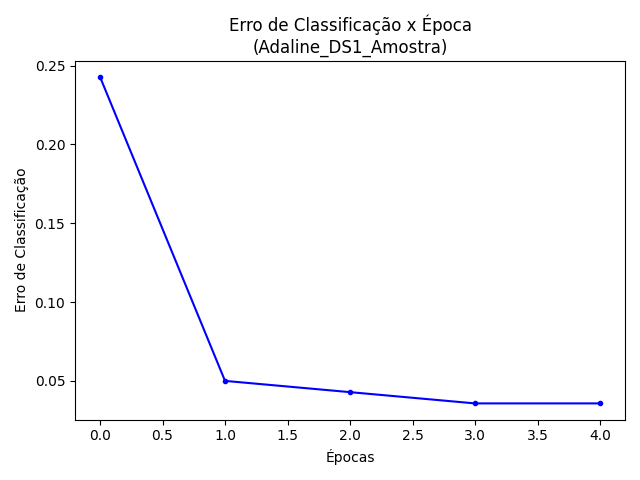
\includegraphics[width=\linewidth]{../../assets/adaline/erro_Adaline_DS1_Amostra.png}
        \caption{Erro de Classif. (Amostra - DS1)}
    \end{minipage}\hfill
    \begin{minipage}{0.48\textwidth}
        \centering
        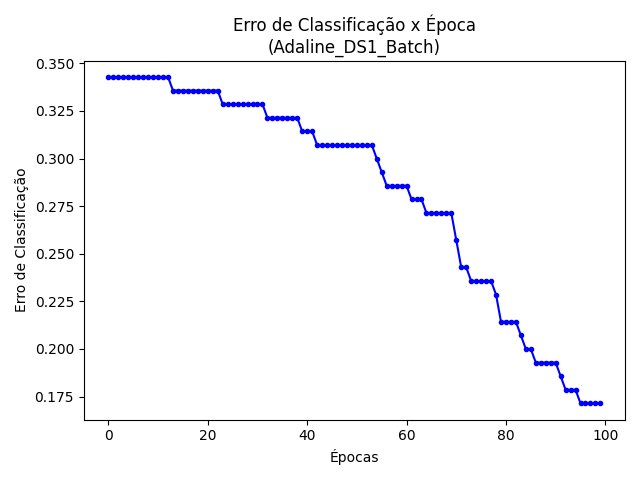
\includegraphics[width=\linewidth]{../../assets/adaline/erro_Adaline_DS1_Batch.png}
        \caption{Erro de Classif. (Batch - DS1)}
    \end{minipage}
\end{figure}

\begin{figure}[H]
    \centering
    \begin{minipage}{0.48\textwidth}
        \centering
        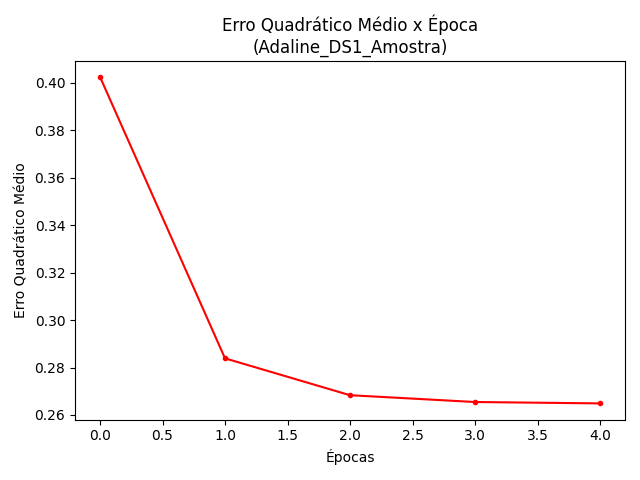
\includegraphics[width=\linewidth]{../../assets/adaline/eqm_Adaline_DS1_Amostra.png}
        \caption{Erro Quadrático (Amostra - DS1)}
    \end{minipage}\hfill
    \begin{minipage}{0.48\textwidth}
        \centering
        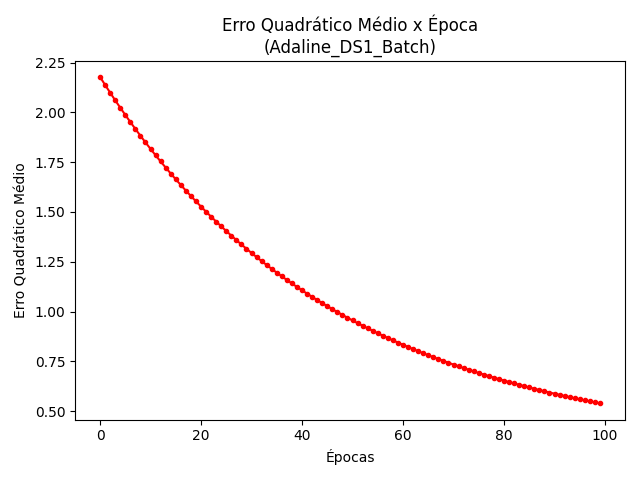
\includegraphics[width=\linewidth]{../../assets/adaline/eqm_Adaline_DS1_Batch.png}
        \caption{Erro Quadrático (Batch - DS1)}
    \end{minipage}
\end{figure}

\subsection{Fronteiras de Decisão (Treino e Teste)}
\begin{figure}[H]
    \centering
    \begin{minipage}{0.48\textwidth}
        \centering
        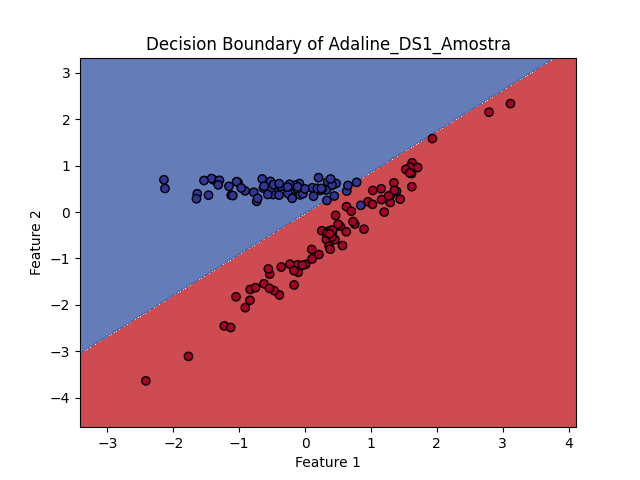
\includegraphics[width=\linewidth]{../../assets/adaline/train_decision_boundary_Adaline_DS1_Amostra.png}
        \caption{Fronteira Treino (Amostra - DS1)}
    \end{minipage}\hfill
    \begin{minipage}{0.48\textwidth}
        \centering
        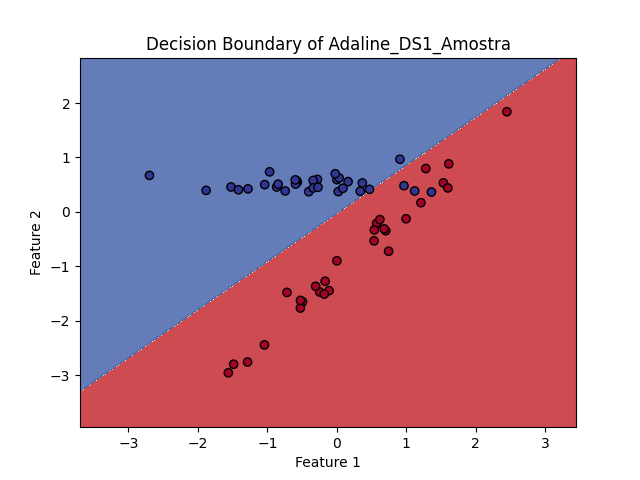
\includegraphics[width=\linewidth]{../../assets/adaline/test_decision_boundary_Adaline_DS1_Amostra.png}
        \caption{Fronteira Teste (Amostra - DS1)}
    \end{minipage}
\end{figure}

\textbf{Discussão (Dataset 1):} Os resultados indicam que o Dataset 1 é amplamente separável linearmente. A abordagem por amostra convergiu muito rapidamente, em apenas 5 épocas, atingindo uma alta acurácia de 96.43\% no treino e 95\% no teste. Por outro lado, o modelo em lote (Batch) precisou de 100 épocas (parada pelo limite máximo) e obteve um desempenho inferior (88.33\% no teste), sugerindo que a taxa de aprendizado de 0.01 pode não ter sido o ajuste ideal para o gradiente médio nesta distribuição específica.


\section{Experimentos: Dataset 2}
O segundo experimento utilizou uma base de 2 atributos com 175 amostras de treino e 75 amostras de teste, mantendo os mesmos hiperparâmetros ($\eta = 0.01$, $\epsilon = 0.001$, máx 100 épocas).

\subsection{Resultados Numéricos}
\begin{table}[H]
\centering
\begin{tabular}{|c|c|c|c|c|}
\hline
\textbf{Abordagem} & \textbf{Épocas} & \textbf{EQM Final} & \textbf{Acc Treino} & \textbf{Acc Teste} \\ \hline
Amostra & 7 & 0.9981 & 45.71\% & 28.00\% \\ \hline
Batch & 100 & 1.2502 & 67.43\% & 70.67\% \\ \hline
\end{tabular}
\caption{Resultados obtidos para o Dataset 2}
\end{table}

\begin{figure}[H]
    \centering
    \begin{minipage}{0.48\textwidth}
        \centering
        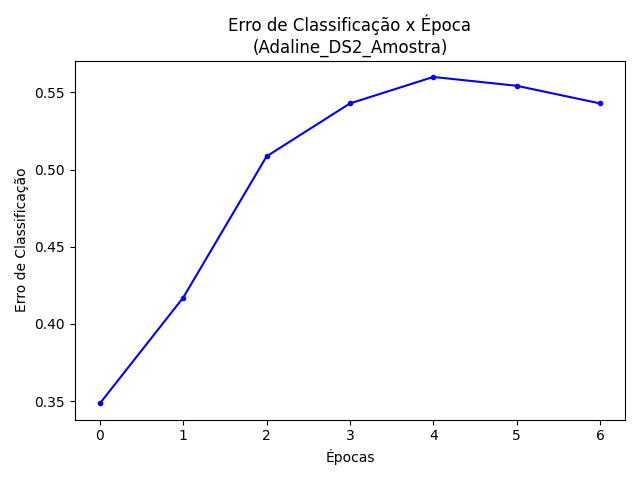
\includegraphics[width=\linewidth]{../../assets/adaline/erro_Adaline_DS2_Amostra.png}
        \caption{Erro de Classif. (Amostra - DS2)}
    \end{minipage}\hfill
    \begin{minipage}{0.48\textwidth}
        \centering
        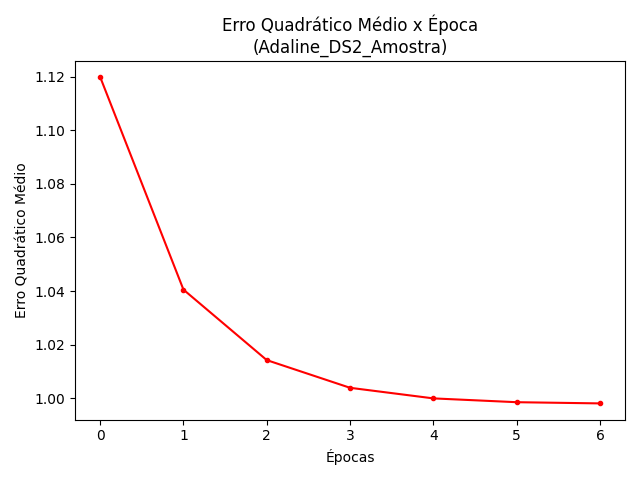
\includegraphics[width=\linewidth]{../../assets/adaline/eqm_Adaline_DS2_Amostra.png}
        \caption{Erro Quadrático (Amostra - DS2)}
    \end{minipage}
\end{figure}

\textbf{Discussão (Dataset 2):} Houve uma nítida dificuldade do modelo em classificar os dados do Dataset 2. A versão por amostra sofreu de convergência prematura em apenas 7 épocas, resultando em métricas extremamente baixas (28\% no teste). A versão em Batch obteve um desempenho ligeiramente melhor e mais coerente (cerca de 70\% de acurácia), esgotando as 100 épocas. A principal conclusão é que, diferentemente do Dataset 1, estes dados possivelmente não são linearmente separáveis ou requerem um ajuste fino de parâmetros e mais épocas para a versão Batch assentar adequadamente a fronteira.


\section{Experimentos: Dataset 3}
O Dataset 3 apresenta maior complexidade, contando com 10 atributos (147 amostras de treino e 63 de teste). Foram avaliadas múltiplas combinações de taxa de aprendizado ($\eta \in \{0.01, 0.001, 0.0001\}$) e critério de parada ($\epsilon \in \{0.1, 0.0001\}$), rodando por até 100 épocas. A fronteira de decisão (gráficos) foi omitida devido à alta dimensionalidade dos dados (>3D).

\subsection{Comparativo de Hiperparâmetros}
\begin{table}[H]
\centering
\resizebox{\textwidth}{!}{
\begin{tabular}{|c|c|c|c|c|c|c|c|}
\hline
\textbf{$\eta$} & \textbf{$\epsilon$} & \textbf{Épocas (Am)} & \textbf{Ac. Treino (Am)} & \textbf{Ac. Teste (Am)} & \textbf{Épocas (Ba)} & \textbf{Ac. Treino (Ba)} & \textbf{Ac. Teste (Ba)} \\ \hline
0.01 & 0.1 & 3 & 93.88\% & 87.30\% & 12 & 60.54\% & 60.32\% \\ \hline
0.01 & 0.0001 & 6 & 93.88\% & 85.71\% & 100 & 78.91\% & 76.19\% \\ \hline
0.001 & 0.1 & 9 & 82.31\% & 76.19\% & 2 & 57.14\% & 57.14\% \\ \hline
0.001 & 0.0001 & 37 & 93.88\% & 88.89\% & 100 & 60.54\% & 60.32\% \\ \hline
0.0001 & 0.1 & 18 & 65.31\% & 63.49\% & 2 & 57.14\% & 57.14\% \\ \hline
0.0001 & 0.0001 & 100 & 84.35\% & 80.95\% & 100 & 57.14\% & 57.14\% \\ \hline
\end{tabular}
}
\caption{Amostra (Am) vs Batch (Ba) no Dataset 3}
\end{table}

\subsection{Análise Gráfica do EQM (Exemplos)}
Abaixo apresentamos gráficos ilustrativos do $E_{qm}$ para diferentes combinações e abordagens:

\begin{figure}[H]
    \centering
    \begin{minipage}{0.48\textwidth}
        \centering
        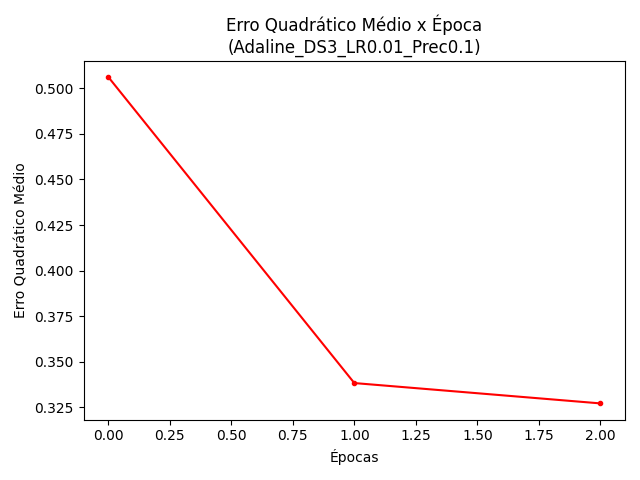
\includegraphics[width=\linewidth]{../../assets/adaline/eqm_Adaline_DS3_LR0.01_Prec0.1.png}
        \caption{EQM: $\eta=0.01, \epsilon=0.1$ (Amostra)}
    \end{minipage}\hfill
    \begin{minipage}{0.48\textwidth}
        \centering
        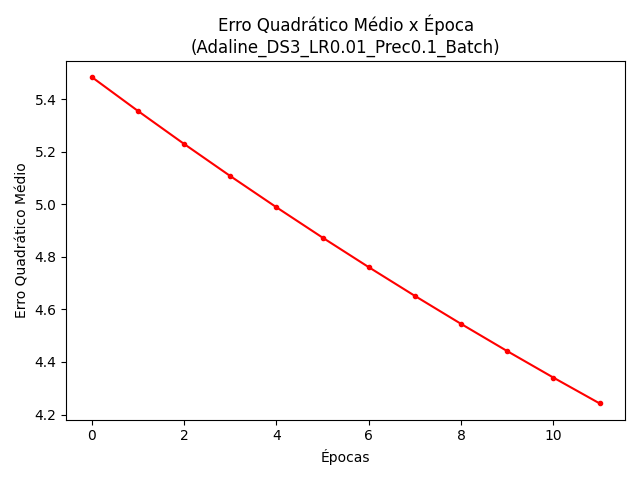
\includegraphics[width=\linewidth]{../../assets/adaline/eqm_Adaline_DS3_LR0.01_Prec0.1_Batch.png}
        \caption{EQM: $\eta=0.01, \epsilon=0.1$ (Batch)}
    \end{minipage}
\end{figure}

\textbf{Discussão (Dataset 3):} A dimensionalidade mais elevada expôs de forma muito clara as diferenças entre os métodos de aprendizado. O método de Amostra obteve resultados de excelência em quase todas as configurações, em especial com $\eta=0.01$ e $\eta=0.001$, beirando 94\% de acurácia em épocas baixas. Por outro lado, o modelo Batch enfrentou severas dificuldades; quando $\epsilon=0.1$, a diferença entre as épocas ficou abaixo da tolerância rapidamente e o treino parou prematuramente (com apenas 2 épocas nos $\eta$ mais baixos). Mesmo quando forçado a rodar 100 épocas (com precisão mais rigorosa), o modelo Batch ficou preso em taxas de acurácia marginais (cerca de 57\% a 60\%). Isso mostra como, em certos cenários multidimensionais com ruído, as atualizações ruidosas amostra por amostra podem ajudar a escapar de mínimos subótimos rasos e encontrar uma solução muito melhor do que o gradiente suave do Batch.

\end{document}
